\documentclass[9pt]{article}

\usepackage{rgstyle}

\usepackage{microtype}
\usepackage{amsmath}
\usepackage{amssymb}
\usepackage{booktabs}
\usepackage{tabularx}
% The template does not configure captions, so they inherit full body size;
% set them one step smaller, as is conventional in conference layouts.
\usepackage[font=small]{caption}
\usepackage{graphicx}
\usepackage{float} % [H]: single-column floats must not float inside multicols
\usepackage{pgf}   % \input{figures/*.pgf} from experiments/make_paper_figures.py
\usepackage{tikz}  % Figure 1 (concept overview); drafted in fig1_draft.tex
\usetikzlibrary{positioning,arrows.meta,calc}
\graphicspath{{figures/}}

% Figure 1 palette (colorblind-safe blue/orange pair; gray is the intentional neutral)
\definecolor{masterblue}{HTML}{2A78D6}
\definecolor{noviceorange}{HTML}{EB6834}
\definecolor{ctrlgray}{HTML}{8A8880}
\definecolor{inksec}{HTML}{52514E}
\definecolor{okgreen}{HTML}{008300}
\definecolor{badred}{HTML}{B3261E}

% Matplotlib's PGF output needs \mathdefault, display-style math and the font
% size it was laid out at (see the header comment in any figures/*.pgf).
% Scoped so none of it leaks into the surrounding document.
\newcommand{\inputpgf}[1]{%
  \begingroup
  \def\mathdefault##1{##1}%
  \everymath=\expandafter{\the\everymath\displaystyle}%
  \fontsize{8}{9.6}\selectfont
  \input{#1}%
  \endgroup
}

\title{Does a Weaker Twin Know Where an LLM's Reasoning Matters?\\
A Causal Test of Master--Novice Divergence\\for Reward Densification}
\setshorttitle{Does a Weaker Twin Know Where an LLM's Reasoning Matters?}

\setauthors{
Ana Carolina Ramos Cunha \quad Leonhard Driesch \quad Leonard Evers
}

\setaffiliations{
School of Computation, Information and Technology \\
Technical University of Munich
}

\setemails{
ana.cunha@tum.de \quad leo.driesch@tum.de \quad ge95gih@mytum.de
}

\date{}

\begin{document}

\setrightlogo{logos/2015_Logo_TUM_sw_RGB.pdf}
\makelogos
\thispagestyle{empty}

\makepapertitle

% --------------------------------------------------
% Abstract
% --------------------------------------------------
\begin{rgabstractbox}
Reinforcement learning for large language models on verifiable tasks (mathematics,
code, and other domains with binary correctness checks) suffers from reward
sparsity: only the final outcome receives a signal, leaving credit assignment
across long chains of thought unresolved. We investigate a Master/Novice
framework that compares a strong policy to a structurally matched but
capacity-reduced \emph{Novice}, obtained by tensor disentanglement of the
Master's MLP weights, and asks whether their per-token divergence identifies
the steps that deserve credit. We contribute (i)~the conceptual framework and
its central, testable hypothesis; (ii)~an end-to-end pipeline that scales
tensor disentanglement to Qwen3.5-4B and bakes Novices at any rank fraction
from a single checkpoint; and (iii)~a hypothesis-first
causal evaluation on MATH-500. Three intervention designs of
increasing strength, namely, handing generation over to the Novice, perturbing single
tokens, and corrupting whole reasoning steps, consistently fail to reject the
null: disagreement positions carry no more outcome leverage than depth-matched
control positions. The only reliable effect is local: disagreement positions are
more fragile in the immediate continuation, and this effect survives
controlling for Master entropy. We report these negative results
precisely, characterize a coherence cliff that constrains usable Novice ranks,
and discuss what they imply for divergence-based reward densification.

\rgkeywords{reinforcement learning, verifiable rewards, credit assignment, tensor disentanglement}
\end{rgabstractbox}

\vspace{1.2em}

% --------------------------------------------------
% Main text
% --------------------------------------------------
\begin{multicols}{2}
\raggedcolumns

% Figure 1: concept overview (drafted standalone in fig1_draft.tex). As a
% full-width float inside multicols it lands at the top of page 2; the
% template's tall abstract box leaves too little room on page 1.
\begin{figure*}[t]
\centering
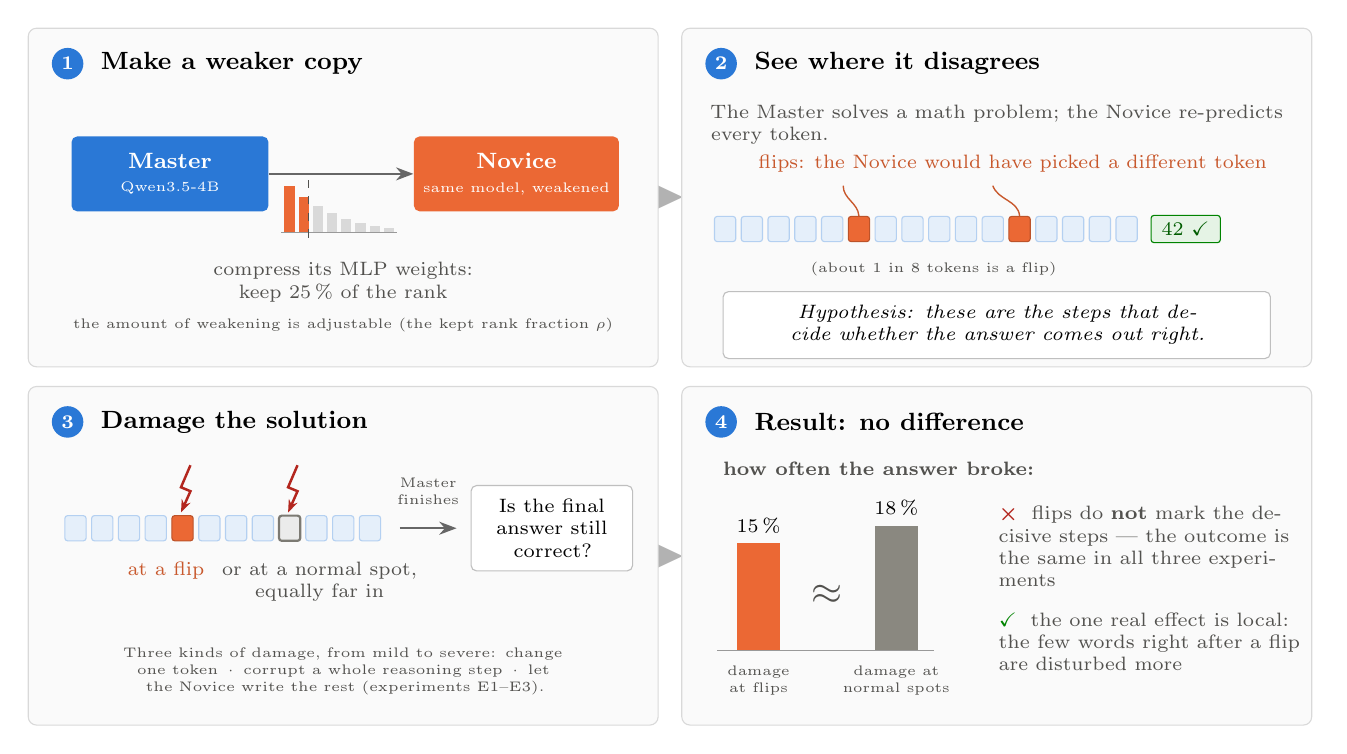
\begin{tikzpicture}[
  x=1cm, y=1cm,
  font=\scriptsize,
  panel/.style={rounded corners=3pt, draw=black!15, fill=black!2},
  num/.style={circle, fill=masterblue, text=white, font=\scriptsize\bfseries,
              inner sep=1.6pt, minimum size=0.4cm},
  ptitle/.style={font=\small\bfseries, anchor=west, text=black},
  modelbox/.style={rounded corners=2pt, minimum width=2.5cm, minimum height=0.95cm,
                   align=center, text=white, font=\footnotesize\bfseries},
  tok/.style={rounded corners=1pt, minimum width=0.27cm, minimum height=0.32cm,
              inner sep=0pt, draw=masterblue!35, fill=masterblue!12},
  flip/.style={tok, draw=noviceorange!80!black, fill=noviceorange},
  ctrl/.style={tok, draw=ctrlgray!90!black, thick, fill=black!8},
  lab/.style={text=inksec, align=left},
  arr/.style={-{Stealth[length=2.2mm]}, thick, black!60},
  bolt/.style={badred, line width=0.9pt, -{Stealth[length=1.6mm]}},
]

% chevrons between panels (reading order 1→2, 3→4)
\node[text=black!30, font=\Large] at (8.15, 6.7)  {$\blacktriangleright$};
\node[text=black!30, font=\Large] at (8.15, 2.15) {$\blacktriangleright$};

% ================= Panel 1 (top left): Make a weaker copy =================
\draw[panel] (0,4.55) rectangle (8.0,8.85);
\node[num] at (0.5,8.4) {1};
\node[ptitle] at (0.8,8.4) {Make a weaker copy};

\node[modelbox, fill=masterblue] (master) at (1.8,7.0)
  {Master\\[-1pt]{\tiny\mdseries Qwen3.5-4B}};

\node[modelbox, fill=noviceorange] (novice) at (6.2,7.0)
  {Novice\\[-1pt]{\tiny\mdseries same model, weakened}};

\draw[arr] (master.east) -- (novice.west);

% singular-spectrum glyph below the arrow, centered in the gap between the boxes
\begin{scope}[shift={($(master.east)!0.5!(novice.west)+(-0.72,-0.75)$)}]
  \foreach [count=\i from 0] \h in {0.60,0.46,0.34,0.25,0.18,0.13,0.09,0.06}{
    \pgfmathsetmacro{\xx}{\i*0.18}
    \ifnum \i<2
      \fill[noviceorange] (\xx,0) rectangle ++(0.13,\h);
    \else
      \fill[black!15] (\xx,0) rectangle ++(0.13,\h);
    \fi
  }
  \draw[black!40, line width=0.4pt] (-0.04,0) -- (1.43,0);
  \draw[dashed, inksec] (0.31,-0.06) -- (0.31,0.7);
\end{scope}

\node[lab, anchor=north, align=center] at (4.0,6.0)
  {compress its MLP weights:\\keep 25\,\% of the rank\\[3pt]
   {\tiny the amount of weakening is adjustable (the kept rank fraction $\rho$)}};

% ================= Panel 2 (top right): See where it disagrees =================
\draw[panel] (8.3,4.55) rectangle (16.3,8.85);
\node[num] at (8.8,8.4) {2};
\node[ptitle] at (9.1,8.4) {See where it disagrees};

\node[lab, anchor=north west, text width=7.6cm] at (8.55,8.0)
  {The Master solves a math problem; the Novice re-predicts every token.};

% token strip
\begin{scope}[shift={(8.85,6.3)}]
  \foreach [count=\i from 0] \s in
    {tok,tok,tok,tok,tok,flip,tok,tok,tok,tok,tok,flip,tok,tok,tok,tok}{
    \node[\s] (t\i) at (\i*0.34,0) {};
  }
  \node[rounded corners=1pt, minimum height=0.32cm, inner sep=2.5pt,
        draw=okgreen, fill=okgreen!10, font=\scriptsize, text=okgreen!70!black]
        (ans) at (15*0.34+0.75,0) {\,$42$ \checkmark\,};
  % flips label above, pointing down
  \node[font=\scriptsize, text=noviceorange!85!black, anchor=south west]
        (flab) at (0.3,0.6)
        {flips: the Novice would have picked a different token};
  \draw[noviceorange!85!black, line width=0.5pt] (1.5,0.55) to[out=-90,in=95] (t5.north);
  \draw[noviceorange!85!black, line width=0.5pt] (3.4,0.55) to[out=-70,in=95] (t11.north);
\end{scope}

\node[lab, font=\tiny, anchor=north, align=center] at (11.5,6.0)
  {(about 1 in 8 tokens is a flip)};

\node[rounded corners=2pt, draw=black!25, fill=white, inner sep=5pt,
      text width=6.6cm, align=center, font=\scriptsize\itshape] at (12.3,5.08)
  {Hypothesis: these are the steps that decide whether the answer comes
   out right.};

% ================= Panel 3 (bottom left): Damage the solution =================
\draw[panel] (0,0) rectangle (8.0,4.3);
\node[num] at (0.5,3.85) {3};
\node[ptitle] at (0.8,3.85) {Damage the solution};

% strip with two damage bolts
\begin{scope}[shift={(0.6,2.5)}]
  \foreach [count=\i from 0] \s in
    {tok,tok,tok,tok,flip,tok,tok,tok,ctrl,tok,tok,tok}{
    \node[\s] (d\i) at (\i*0.34,0) {};
  }
  % lightning bolts onto the flip and the control token
  \draw[bolt] (1.46,0.80) -- (1.34,0.52) -- (1.46,0.47) -- (1.34,0.20);
  \draw[bolt] (2.82,0.80) -- (2.70,0.52) -- (2.82,0.47) -- (2.70,0.20);
  % labels under the strip
  \node[font=\scriptsize, text=noviceorange!85!black, anchor=north, align=center]
    at (1.15,-0.3) {at a flip};
  \node[font=\scriptsize, text=inksec, anchor=north, align=center]
    at (3.1,-0.3) {or at a normal spot,\\equally far in};
\end{scope}

\draw[arr] (4.72,2.5) -- (5.44,2.5);
\node[lab, font=\tiny, anchor=south, align=center] at (5.08,2.68) {Master\\finishes};

\node[rounded corners=2pt, draw=black!25, fill=white, inner sep=5pt,
      text width=1.7cm, align=center, font=\scriptsize] at (6.65,2.5)
  {Is the final answer still correct?};

\node[lab, font=\tiny, anchor=north, align=center, text width=7.4cm] at (4.0,1.1)
  {Three kinds of damage, from mild to severe: change one token \,$\cdot$\,
   corrupt a whole reasoning step \,$\cdot$\, let the Novice write the rest
   (experiments E1--E3).};

% ================= Panel 4 (bottom right): Result =================
\draw[panel] (8.3,0) rectangle (16.3,4.3);
\node[num] at (8.8,3.85) {4};
\node[ptitle] at (9.1,3.85) {Result: no difference};

\node[lab, font=\scriptsize\bfseries, anchor=west] at (8.7,3.25)
  {how often the answer broke:};

\begin{scope}[shift={(9.0,0.95)}]
  % bars: E3 break rates .151 vs .176, scale x9
  \draw[black!40, line width=0.4pt] (-0.25,0) -- (2.5,0);
  \fill[noviceorange] (0,0)   rectangle ++(0.55,{0.151*9});
  \fill[ctrlgray]     (1.75,0) rectangle ++(0.55,{0.176*9});
  \node[font=\scriptsize, anchor=south] at (0.275,{0.151*9}) {15\,\%};
  \node[font=\scriptsize, anchor=south] at (2.025,{0.176*9}) {18\,\%};
  \node[font=\Large, text=inksec] at (1.15,0.7) {$\approx$};
  \node[font=\tiny, text=inksec, anchor=north, align=center] at (0.275,-0.08)
    {damage\\at flips};
  \node[font=\tiny, text=inksec, anchor=north, align=center] at (2.025,-0.08)
    {damage at\\normal spots};
\end{scope}

\node[lab, anchor=north west, text width=3.9cm] at (12.2,2.9)
  {\textcolor{badred}{$\boldsymbol\times$}\; flips do \textbf{not} mark the
   decisive steps --- the outcome is the same in all three experiments};

\node[lab, anchor=north west, text width=3.9cm] at (12.2,1.55)
  {\textcolor{okgreen}{\checkmark}\; the one real effect is local: the few
   words right after a flip are disturbed more};

\end{tikzpicture}
\caption{What we did and what we found: \textbf{(1)}~compress a strong model's
(\emph{Master's}) MLP weights into a weakened copy, the \emph{Novice};
\textbf{(2)}~let the Novice re-predict the Master's correct MATH-500
solutions and mark the disagreements (\emph{flips}); \textbf{(3)}~damage
solutions at flips versus at depth-matched normal positions and let the
Master finish. \textbf{(4)}~\emph{Takeaway:} the answer breaks equally often
either way (shown: whole-step damage; all three experiments agree), so flips
mark where the Novice's missing capacity acts --- not where the outcome is
decided --- and this divergence signal cannot densify the reward.}
\label{fig:overview}
\end{figure*}


% --------------------------------------------------
\section{Introduction}

A large language model (LLM) that solves a competition-mathematics problem
under reinforcement learning emits hundreds of chain-of-thought tokens and
then receives a single bit of reward: the final answer checks out or it does
not. That bit credits every step equally, although a few steps decide the
outcome and most are routine. Which steps deserved the credit is exactly what
the policy cannot see, and this unresolved credit assignment is a chief cost
of reward sparsity in verifiable-reward RL~\citep{cui2025prime}.

Existing densification methods mine structure already present in the task or
the model, from partial test-case success to token entropy
(Section~\ref{sec:related}). This paper explores a complementary idea: construct a weaker \emph{Novice} from
the same base weights as the \emph{Master} via tensor disentanglement, compare
their next-token distributions on successful Master rollouts, and upweight
positions where the two diverge, on the premise that such steps rely on
knowledge the Novice lacks and therefore deserve higher credit. Unlike an
externally trained reward model, the Novice shares architecture and tokenizer
with the Master and offers a continuous knob (the retained rank fraction) for
how weak the comparator should be. Figure~\ref{fig:overview} summarizes the
approach and its outcome.

Our contributions are of three kinds. \emph{Conceptually}, we formalize the
Master/Novice framework and reduce its promise to a single testable hypothesis:
divergence positions have higher causal leverage on the final outcome than
matched non-divergence positions. \emph{Methodologically}, we implement an
end-to-end pipeline that disentangles a base model, persists the factors,
bakes a Novice at any chosen rank, and generates, together with a ladder of
three causal intervention designs for testing per-token credit signals before
committing to RL training.
\emph{Empirically}, we characterize the disentanglement and Novice-quality
landscape (learning-rate sweep, MMLU rank sweep, a generation-level coherence
cliff) and report a consistent, statistically quantified negative result on the
central hypothesis, alongside one genuine positive: a local fragility effect at
disagreement positions that is not explained by Master entropy alone.

% --------------------------------------------------
\section{Related Work}\label{sec:related}

We group prior work by where the dense signal comes from: the \emph{task}
(verifiable structure) or the \emph{model} (internal statistics). For each line
of work we focus on its relation to our approach; we refer to the original
papers for full results.

\subsection{Dense rewards from verifiable task structure}

\textbf{VeRPO}~\citep{wang2026verpo} densifies code-RL rewards using partial
test-case success. Its central observation is cautionary: the naive dense
signal (the raw test-suite pass rate) can \emph{underperform} sparse outcome
rewards, because redundant easy tests dominate the reward by sheer count (a
\emph{cardinality bias}). VeRPO corrects this with a dynamically calibrated
per-test weighting and re-anchors the result to the end-to-end outcome,
outperforming outcome-only
GRPO~\citep{shao2024deepseekmathpushinglimitsmathematical} and RM-based
baselines without a learned
reward model. VeRPO is the clearest instance of extracting density from the
\emph{verifier} side, and its lesson that denser is not automatically better
motivates our causal validation of the divergence signal before any
training. The approach differs from ours in
scope and granularity: the signal exists only where partial success is
measurable (currently code) and is assigned per turn, whereas a Master/Novice
comparator is task-agnostic and per token.

\textbf{PRIME}~\citep{cui2025prime} obtains per-token process rewards without
step labels by training an outcome reward model whose log-ratio to a reference
policy is reinterpreted as an implicit process reward, updated online alongside
the policy. It substantially improves sample efficiency over outcome-only RL on
math and code. PRIME is the closest point of comparison for our goal
(token-level credit from outcome supervision only); the difference is that
PRIME \emph{learns} its dense signal, whereas we test whether a fixed,
training-free capacity-reduced copy of the policy can supply one. Supervised
process reward models reach the same per-step granularity by training on
explicit step labels, human-annotated~\citep{lightman2023letsverify} or
constructed automatically from per-step completion
success~\citep{wang2023mathshepherd}; a training-free comparator sits at the
opposite end of this supervision spectrum.

\subsection{Token-importance signals inside the model}

\textbf{High-entropy minority tokens.} \citet{wang2025forking} show that in RLVR most chain-of-thought tokens are
low-entropy ``followers,'' while a minority of high-entropy forking tokens
carries the learning signal: restricting policy gradients to the top 20\%
highest-entropy tokens matches or exceeds full-gradient training. Master
entropy is thus the natural single-model baseline that any two-model
divergence signal must beat; our experiments therefore control for entropy
explicitly.

\textbf{TIP}~\citep{xu2026tip} studies on-policy distillation and identifies
informative tokens along two axes, student entropy and teacher-student
divergence: entropy-only selection is structurally blind to positions where
the student is confidently wrong, and training on under 10\% of tokens, from the
low-entropy, high-divergence region alone, nearly matches full-token
distillation. TIP is the closest conceptual
relative of our hypothesis in the sense that divergence between a strong and a weak model marks
important tokens, but it operates in distillation, where the teacher's
distribution is the training target itself. Whether the same signal identifies
\emph{outcome-critical} steps for RL credit assignment is exactly the question
our experiments address.

Compared with all four, the Master/Novice comparator is training-free: no
reward model, no step labels, no verifier beyond the outcome check, just a
second forward pass. But training-free does not mean trustworthy. The rest
of this paper tests whether its signal marks the right tokens.

% --------------------------------------------------
\section{Methodology}

\subsection{Setup and hypothesis}\label{sec:hypothesis}

We treat autoregressive generation as a Markov decision process: state $s_t$ is
the prompt plus generated prefix $y_{<t}$, action $a_t$ is the next token, and
the reward is binary verifiable correctness at episode end. The
\textbf{Master} is the full-capacity policy $\pi_M$. The \textbf{Novice} is
$\pi_N$, derived from the same checkpoint by truncating disentangled MLP
factors to a rank fraction $\rho \in (0,1]$, the share of each layer's internal
rank that is kept (defined precisely in Section~\ref{sec:wmd}); $\rho{=}1$
reproduces the Master and smaller $\rho$ yields a weaker Novice. On a Master
rollout $\tau = (y_1,\ldots,y_T)$ that reaches a correct answer, the
framework scores each position by how much the two next-token distributions
$\pi_M(\cdot \mid y_{<t})$ and $\pi_N(\cdot \mid y_{<t})$ diverge; any
divergence measure qualifies, e.g.\ Kullback--Leibler (KL) or
Jensen--Shannon. Our experiments use the simplest instantiation, the
parameter-free \emph{top-1 flip}: a position counts as a flip when the
Novice's most probable next token differs from the token the Master actually
emitted there, i.e., when the Novice, sampling greedily, would have written
something else. This setup, where the full
policy generates while its truncated counterpart re-scores the same
states, instantiates the \emph{Observer pattern} of the introspection
framework of \citet{till2026introspection},
and the top-1 flip corresponds to its discrete \emph{behavioral disagreement}
indicator.

The intended use of this divergence signal is as a shaping weight that
concentrates credit on high-divergence steps of verified-correct rollouts. Before such a signal
enters any RL objective, however, its premise must hold. We therefore state it
as an explicit hypothesis:

\medskip
\noindent\textbf{H1 (outcome leverage).} \emph{Positions where the Novice
diverges from the Master have a larger causal effect on final-answer
correctness than depth-matched positions where the two agree.}
\medskip

\noindent All credit-assignment experiments in this paper are direct causal
tests of H1 at increasing intervention strength. We deliberately do not
evaluate any RL training run: if H1 fails, divergence-weighted advantages
cannot concentrate gradient where the outcome is decided, and the training
experiment would be uninformative.

\subsection{Constructing the Novice via weight matrix disentanglement}\label{sec:wmd}

The Novice must be \emph{policy-preserving}: it should retain as much of the
Master's behavior as a given rank budget permits, so that its remaining
disagreements are attributable to missing capacity rather than to a lossy
construction. The classical route, truncated SVD of each weight matrix, treats the matrix as a flat 2D
array and ignores the multi-dimensional structure of neural weights. We
instead use the \emph{Weight Matrix Disentanglement} (WMD) of
\citet{till2026introspection}, which adapts tensor disentanglement from
numerical linear algebra~\citep{wei2025tensor} to neural network layers.

Let $X \in \mathbb{R}^{lr \times bc}$ be a decoder-MLP weight matrix whose row
and column counts are each written as a product of two integers, $lr$ split
into the near-balanced pair $(l, r)$ and $bc$ into $(b, c)$; this lets the flat
matrix be read as a four-index tensor rather than a 2D array, which is what
exposes the multi-dimensional structure that plain SVD ignores. Writing $M$ for
the reshape of $X$ into the 4th-order tensor
$\mathcal{X} \in \mathbb{R}^{l \times r \times b \times c}$ and $P$ for the
index permutation $(l,r,b,c) \to (l,c,r,b)$, WMD re-bipartitions the tensor
with the operator
\begin{equation}
A \equiv M^{-1} \circ P \circ M \colon\;
\mathbb{R}^{lr \times bc} \to \mathbb{R}^{lc \times rb},
\end{equation}
exposing cross-dimensional correlations that the flat matricization hides. Before the re-bipartitioning, a learnable orthogonal matrix
$Q \in O(lr)$ (the orthogonal group) is applied to the row space. We call
$Q$ a \emph{gauge} because reconstruction later undoes it with $Q^{\top}$:
it re-expresses the layer's coordinates without changing the layer itself.
The gauge is optimized to concentrate the spectrum of $A(QX)$ in its leading
singular directions, i.e., to make a few large singular values carry most of
the energy. For a target rank $k$, the optimal
disentangler minimizes the energy of the discarded singular tail:
\begin{equation}
Q^{*}_{k} \;=\; \operatorname*{arg\,min}_{Q \in O(lr)}
\sum_{i > k} \sigma_i^2\bigl(A(QX)\bigr).
\label{eq:gauge}
\end{equation}
The tail sum $\sum_{i>k}\sigma_i^2$ is exactly the squared error of replacing
$A(QX)$ by its best rank-$k$ approximation, so a gauge that shrinks it makes
the layer more compressible. Because $A$ is an isometry (a norm-preserving
map) and $Q$ is orthogonal, the total singular energy of $A(QX)$ is invariant,
so \eqref{eq:gauge} directly minimizes the Frobenius reconstruction error (the
sum of squared entrywise differences) between the original and truncated
layer; the identity gauge $Q{=}I$
recovers plain SVD truncation, so the optimized gauge is never worse. The
rank-$k$ Novice weight is reconstructed by inverting the pipeline,
\begin{equation}
\widetilde{X}^{(k)} \;=\; Q^{*\top}
A^{-1}\bigl(\operatorname{trunc}_k(A(Q^{*}X))\bigr),
\label{eq:bake}
\end{equation}
and the per-layer rank is set by a single global rank fraction:
$k(\rho) = \max(1, \lceil \rho\, m \rceil)$, where $m = \min(lc, rb)$ is the
largest possible rank of $A(QX)$. Thus $\rho$ is literally the fraction of
singular directions kept, and the outer $\max$ with 1 guarantees at least one
is retained.

Concretely, for Qwen3.5-4B's \texttt{down\_proj} (one of the three MLP
projection matrices in each decoder layer, here
$X \in \mathbb{R}^{2560 \times 9216}$) the factorization is
$(l,r,b,c) = (40,64,96,96)$, so that $40 \times 64 = 2560$ and
$96 \times 96 = 9216$ recover the matrix dimensions; then $Q \in O(2560)$,
$A(QX) \in \mathbb{R}^{3840 \times 6144}$, and $m = 3840$, so baking at
$\rho{=}0.25$ keeps $k{=}960$ singular directions. The stored per-layer
factors $(Q, U, s, V_h)$, namely the gauge together with the singular vectors
and values $U$, $s$, $V_h$ of $A(Q^{*}X)$, retain the full decomposition, so
one disentanglement run yields Novices at every $\rho$ by cheap
re-truncation; an equality test confirms that a Novice baked at $\rho{=}1$
reproduces the base model's logits (implementation details in
Appendix~\ref{app:repro}).

The optimization problem \eqref{eq:gauge} admits a closed-form gradient that
reuses one SVD of $A(QX)$ per step~\citep{wei2025tensor}. Our implementation
(based on the reference disentanglement code) accelerates this optimization
by roughly 30--50$\times$ per layer while keeping truncation cost within
$\sim$10\% of the double-precision reference, which is what makes
constructing Novices at the 4B scale of our experiments practical; the
individual optimizations are described in Appendix~\ref{app:repro}.

WMD also supplies the theoretical link between Novice construction and the
divergence signal of Section~\ref{sec:hypothesis}: for a policy and its rank-$k$ truncated
counterpart, the per-state KL divergence is bounded by the discarded singular
tail, $D_{\mathrm{KL}}\bigl(\pi_M(\cdot \mid s)\,\|\,\pi_N(\cdot \mid s)\bigr)
\le \tfrac{L}{2} \sum_{i>k} \sigma_i^2\bigl(A(Q^{*}X)\bigr)$ with $L$ a
network-wide Fisher-information Lipschitz constant, a fixed factor that
converts discarded weight energy into a bound on how much the output
distribution can change~\citep{till2026introspection}. Because baking
truncates the stored factors of $A(Q^{*}X)$, exactly the construction in
\eqref{eq:bake}, the bound holds at every bake rank $\rho$; its
\emph{tightness}, however, is only guaranteed at the rank the gauge was
optimized for, since \eqref{eq:gauge} depends on $k$. We verify empirically
that the gauge's advantage transfers across ranks in our checkpoint
(Section~\ref{sec:characterization}). WMD rather than plain SVD
thus keeps the observed Master/Novice divergence dominated by genuinely
missing capacity rather than by avoidable truncation error.

% --------------------------------------------------
\section{Experiments}

\subsection{Models, data, and grading}

\textbf{Models.} Master: \texttt{Qwen/Qwen3.5-4B}~\citep{qwen35blog} at full
rank. Novice: the
disentangled checkpoint of the same model (gauge optimized at $\rho{=}0.1$),
baked at $\rho{=}0.25$; the bake-rank choice is justified empirically in
Section~\ref{sec:characterization}.

\textbf{Data.} MATH-500~\citep{lightman2023letsverify}, a 500-problem subset
of the MATH
dataset~\citep{hendrycks2021measuringmathematicalproblemsolving}, restricted to the
first 50 problems (0--49) to fit our compute budget,
prompted via the chat template with the standard instruction to place the
final answer in \texttt{\textbackslash boxed\{\}}. All decoding is greedy;
Master rollouts are capped at 512 new tokens in E1 and 700 in E2/E3 (under
greedy decoding the shared prefixes are identical, and the same 23 problems
are solved), which sufficed for most rollouts to terminate naturally. Greedy
decoding makes every experiment deterministic up to the
fixed sampling seed used for control selection.

\textbf{Grading.} A rollout counts as correct when its extracted
\texttt{\textbackslash boxed\{\}} answer matches the reference after LaTeX
normalization (extractor details in Appendix~\ref{app:repro}). The Master
solved 23/50 problems; all
credit-assignment experiments operate on these 23 verified-correct rollouts.
Across them, the Novice is teacher-forced on the Master's tokens and flips are
recorded at every generated position (10{,}895 scored tokens; flip rate
12.3\%). The disentangled factor checkpoint is publicly available, and
Appendix~\ref{app:repro} collects all remaining reproduction details (seeds,
prompts, evaluation configuration); code and per-trial artifacts are
available from the authors.

\subsection{Intervention experiments}

All three experiments compare \emph{flip} positions against \emph{depth-matched
non-flip controls}. The \emph{depth} of a position is its relative location
within the generated part of the rollout, from 0 (first generated token) to 1
(last). Depth matching is essential because an intervention late in a rollout
is much easier to recover from, since most of the correct solution is already
in place; how far into a rollout an intervention occurs in fact dominates its
effect (Section~\ref{sec:intervention-results}), so comparisons at unmatched
depths would be confounded. Controls are drawn once per flip with a fixed
random seed. Figure~\ref{fig:designs} summarizes the three designs.

% Figure: the three intervention designs E1--E3 as compact dot-path
% sketches (blue: Master, orange: flip/Novice, gray: control/abandoned).
% [H] floats cannot float inside multicols, so this \input is placed
% manually where the figure fits without leaving a column gap.
\begin{figure}[H]
\centering
\resizebox{\linewidth}{!}{%
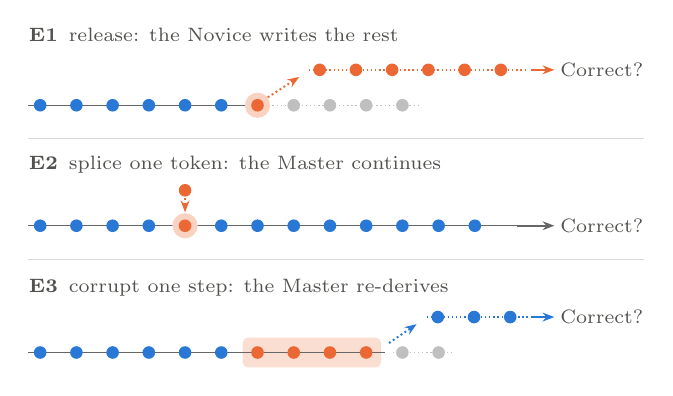
\begin{tikzpicture}[
  x=1cm, y=1cm,
  font=\scriptsize,
  lab/.style={text=inksec, anchor=west, font=\scriptsize, inner sep=0pt},
  branch/.style={densely dotted, line width=0.7pt, -{Stealth[length=1.5mm]}},
]

% ---- E1: release-from-here. Novice branch (orange) takes over at the
% flip; the Master's own continuation is abandoned (gray).
\node[lab] at (0,3.9) {\textbf{E1}\enspace release: the Novice writes the rest};
\draw[black!60, line width=0.5pt] (0,3.0) -- (2.97,3.0);
\draw[black!25, densely dotted, line width=0.5pt] (3.1,3.0) -- (4.95,3.0);
\foreach \i in {0,...,5} \fill[masterblue] (0.15+\i*0.46,3.0) circle (0.08);
\fill[noviceorange!30] (2.91,3.0) circle (0.16);
\fill[noviceorange]    (2.91,3.0) circle (0.08);
\foreach \i in {7,...,10} \fill[black!25] (0.15+\i*0.46,3.0) circle (0.08);
\draw[branch, noviceorange] (3.04,3.1) -- (3.44,3.36);
\draw[noviceorange, densely dotted, line width=0.5pt] (3.56,3.45) -- (6.35,3.45);
\foreach \i in {0,...,5} \fill[noviceorange] (3.7+\i*0.46,3.45) circle (0.08);
\draw[-{Stealth[length=1.5mm]}, noviceorange, line width=0.6pt]
  (6.38,3.45) -- (6.68,3.45);
\node[lab] (correctlabel) at (6.75,3.45) {Correct?};

% ---- separator between E1 and E2
\draw[black!15, line width=0.4pt] (0,2.58) -- (correctlabel.east |- 0,2.58);

% ---- E2: single-token perturbation. A token is spliced in from above
% at the flip; the Master continues.
\node[lab] at (0,2.25) {\textbf{E2}\enspace splice one token: the Master continues};
\draw[black!60, line width=0.5pt] (0,1.47) -- (6.2,1.47);
\draw[-{Stealth[length=1.5mm]}, black!60, line width=0.6pt]
  (6.2,1.47) -- (6.68,1.47);
\foreach \i in {0,1,2,3,5,6,7,8,9,10,11,12}
  \fill[masterblue] (0.15+\i*0.46,1.47) circle (0.08);
\fill[noviceorange!30] (1.99,1.47) circle (0.16);
\fill[noviceorange]    (1.99,1.47) circle (0.08);
\fill[noviceorange] (1.99,1.92) circle (0.08);
\draw[branch, noviceorange] (1.99,1.82) -- (1.99,1.64);
\node[lab] at (6.75,1.47) {Correct?};

% ---- separator between E2 and E3
\draw[black!15, line width=0.4pt] (0,1.04) -- (correctlabel.east |- 0,1.04);

% ---- E3: span perturbation. A whole step is corrupted (orange band);
% the Master free-runs afterwards (blue branch), abandoning its
% original continuation (gray).
\node[lab] at (0,0.68) {\textbf{E3}\enspace corrupt one step: the Master re-derives};
\fill[noviceorange!22, rounded corners=2pt] (2.72,-0.33) rectangle (4.48,0.05);
\draw[black!60, line width=0.5pt] (0,-0.14) -- (4.53,-0.14);
\draw[black!25, densely dotted, line width=0.5pt] (4.63,-0.14) -- (5.4,-0.14);
\foreach \i in {0,...,5} \fill[masterblue] (0.15+\i*0.46,-0.14) circle (0.08);
\foreach \i in {6,...,9} \fill[noviceorange] (0.15+\i*0.46,-0.14) circle (0.08);
\foreach \i in {10,11} \fill[black!25] (0.15+\i*0.46,-0.14) circle (0.08);
\draw[branch, masterblue] (4.58,-0.02) -- (4.93,0.22);
\draw[masterblue, densely dotted, line width=0.5pt] (5.06,0.31) -- (6.35,0.31);
\foreach \i in {0,1,2} \fill[masterblue] (5.2+\i*0.46,0.31) circle (0.08);
\draw[-{Stealth[length=1.5mm]}, masterblue, line width=0.6pt]
  (6.38,0.31) -- (6.68,0.31);
\node[lab] at (6.75,0.31) {Correct?};

\end{tikzpicture}%
}
\caption{The three intervention designs on a Master rollout (dots:
tokens; orange marks the flip the intervention strikes).
\textbf{E1} releases the Novice at the flip: it writes the rest (orange
path) and the Master's continuation is abandoned (gray); \textbf{E2}
splices in a single token and the Master continues; \textbf{E3}
corrupts a whole flip-dense step (orange band), after which the Master
free-runs (blue path) instead of following its original continuation
(gray). Every trajectory is re-graded (``Correct?''), and every
intervention is repeated at a depth-matched control position (not
shown). H1 predicts more broken answers at flips than at controls;
Section~\ref{sec:intervention-results} finds no such difference at any
granularity.}
\label{fig:designs}
\end{figure}


\textbf{E1: Release-from-here.} At a chosen position $p$ the Novice takes over:
it receives the Master's prefix $y_{<p}$ and free-runs greedily to completion
(budget: remaining rollout length plus 48 tokens); the completed trajectory is
graded. This mirrors the deployment (``Actor'') pattern of the WMD
framework~\citep{till2026introspection}, in which the truncated policy drives
the rollout. Release positions are selected as follows. Within each rollout,
all flips are ranked by their \emph{confidence gap}: the probability the
Novice assigns to its own preferred token minus the probability it assigns to
the Master's token at that position. A near-zero gap means a borderline
disagreement, a large gap a confident one. We release at the 5 most confident
flips per rollout, since these are the flips most likely to matter if H1 is
true; selecting them biases the test toward finding an effect, which makes a
null result more conclusive. Each selected flip is then paired with the
not-yet-used non-flip position closest to it in depth, and every control is
used at most once. With 23 rollouts and 5 pairs each, this yields
$23 \times 5 = 115$ pairs, i.e., 230 Novice free-runs; five pairs per rollout
balance per-problem coverage against generation cost. If H1 holds, releasing
at a flip should derail the answer more often than at its matched control.

\textbf{E2: Single-token perturbation.} E1 is a coarse test: after the
handoff a whole weak model free-runs, so in both arms the one-token
difference at the release position is swamped by hundreds of subsequent
Novice-generated tokens. E2 instead perturbs exactly one token and lets the
\emph{Master} continue. It asks two questions that E1 cannot separate: does
the \emph{position} of a flip matter, and does the Novice's \emph{specific
token} matter beyond a generic error at that position?

Three arms, built from the same 5 flip/control pairs per rollout as E1,
answer these questions. \texttt{flip\_novice} splices the Novice's token at
the flip position. \texttt{flip\_rank2} splices the Master's own second most
probable token at the same flip position. \texttt{control\_rank2} splices the
second-choice token at the matched control position. The second-choice token
serves as the generic perturbation because it exists at every position and is
comparably strong at flip and control positions alike. \texttt{flip\_rank2}
is the arm shared by both comparisons: against \texttt{control\_rank2} it
isolates the position effect under an identical perturbation type, and
against \texttt{flip\_novice} it isolates the effect of the Novice's specific
token at an identical position. (The fourth combination, the Novice's token
at a control position, cannot exist: at a non-flip position the Novice's
token \emph{is} the Master's.) Each of the 115 pairs thus produces three
trials, for $23 \times 5 \times 3 = 345$ in total, 115 per arm.

Three metrics are recorded per trial. (i)~\emph{Local disruption}: the mean
drop in the log-probability the Master assigns to its own next $K{=}8$
tokens when the perturbed prefix replaces the clean one, in nats per token.
A drop of one nat means the Master finds its own continuation a factor of
$e$ less likely; $K{=}8$ captures the immediate continuation while keeping
the metric local. (ii)~\emph{Answer log-probability drop}: the same drop
evaluated on the Master's answer tokens (the
\texttt{\textbackslash boxed\{\}} content), with the reasoning between the
perturbation and the answer teacher-forced, i.e., held fixed. This isolates
the part of the perturbation's effect that reaches the outcome; trials whose
perturbed position lies after the answer span have no answer tokens left to
score and are excluded. (iii)~A binary \emph{answer-break} outcome: whether
the Master, free-running greedily from the perturbed prefix, no longer
reaches the correct answer. Each free-run is a full generation, so this
metric is evaluated on a random subset of 90 of the 345 trials to bound
compute.

Position comparisons face a confound: flips concentrate at positions where
the Master itself is uncertain, and perturbing an uncertain position
disturbs the continuation more for purely mechanical reasons. All position
comparisons are therefore additionally adjusted for entropy by ordinary
least squares, $y = \beta_0 + \beta_1\,\mathrm{isflip} + \beta_2\,H_M$,
where $\mathrm{isflip}$ indicates a flip position and $H_M$ is the Shannon
entropy (in nats) of the Master's next-token distribution at the perturbed
position. The regression is fitted over the two \texttt{rank2} arms only, so
that both arms received the identical perturbation type; $\beta_1$ then
estimates the difference between a flip and a control position at equal
entropy.

\textbf{E3: Span perturbation.} Single tokens may be the wrong granularity for
reasoning. E3 corrupts an entire reasoning step, simplified here as a newline-delimited token
span. Spans shorter than 4 tokens are discarded as trivial fragments. It then
lets the Master free-run to the answer, so the downstream reasoning may adapt.
Steps are ranked by \emph{flip density}, the fraction of their tokens that
are flips; per rollout the 3 densest steps are paired with depth-matched
low-density steps (three per rollout, for the same coverage-cost balance as
in E1), giving $23 \times 3 = 69$ step pairs. Arms mirror E2: generic
corruption (per-position second-choice tokens) of a flip-dense step, generic
corruption of a control step, and replacement of the flip-dense step by the
\emph{Novice's version} of it (its preferred token at every position), for
$69 \times 3 = 207$ trials in total, 69 per arm. The primary metric is the
binary answer-break rate of the Master's free-run, evaluated on 150 of the
207 trials; the teacher-forced answer drop and the entropy-adjusted
regression (with the step's mean entropy as covariate) are reported as in E2,
where one step pair without answer tokens after the span is excluded.

\textbf{Statistical analysis.} We attach a standard test to each comparison so
that a null result can be quantified rather than merely asserted. Every rate
is reported with a 95\% Wilson confidence interval (CI). E1's flip and control
arms are \emph{paired}, since each flip has its own depth-matched control, and
are compared with McNemar's exact test; E2 and E3 treat their free-run arms as
\emph{independent} groups, compared with Fisher's exact test, whose
\emph{odds ratio} is above 1 when the flip arm broke the answer more often.
For the regression coefficients $\beta_1$ and $\beta_2$ we report the
estimate, its standard error (SE), and the $t$-value (estimate divided by
SE); at our sample sizes $|t| \gtrsim 2$ corresponds to $p \lesssim 0.05$.
Appendix~\ref{app:stats} explains each test and why it matches the design. In
every case a small $p$-value, a $t$-value past this threshold, or a CI that
excludes the no-effect value would signal a real effect; as the next section
shows, we observe none of these.

% --------------------------------------------------
\section{Results}

\subsection{Novice characterization}\label{sec:characterization}

\textbf{Learning-rate selection.} Disentanglement quality is sensitive to the
optimizer learning rate; a sweep on a representative Qwen3.5-4B MLP layer
selects $10^{-3}$, used for all disentanglement runs in the paper
(Appendix~\ref{app:lr}).

\textbf{Gauge quality across bake ranks.} The checkpoint's gauge was optimized
at $\rho{=}0.1$ while the interventions bake at $\rho{=}0.25$, so the KL
bound's tightness is not guaranteed at the bake rank
(Section~\ref{sec:wmd}). Measured on the stored spectra, the advantage
transfers: the optimized gauge's reduction of discarded tail energy relative
to identity-gauge (plain SVD) truncation is large, if heterogeneous across
layers, and essentially rank-independent between $\rho{=}0.1$ and
$\rho{=}0.25$ (Appendix~\ref{app:gauge}).

\textbf{MMLU vs.\ rank.} Novice quality as a function of $\rho$ is measured
with \texttt{lm-eval}~\citep{eval-harness} on
MMLU~\citep{hendrycks2021measuringmassivemultitasklanguage}, 5-shot, limited
to 5 questions per subtask (the same fixed-budget protocol at every rank, so
relative comparisons are unaffected by the limit). Accuracy stays near the
base model's 0.737 down to $\rho \approx 0.5$, then degrades monotonically to
0.42 at $\rho{=}0.1$: still above the 0.25 random baseline
(Figure~\ref{fig:mmlu}).

\textbf{Coherence cliff.} Because MMLU scores likelihood ranking rather than
generation, we separately inspect greedy free-running generations of the
Novice at $\rho \in \{0.1, 0.25, 0.5, 0.75\}$ on MATH-500 prompts. These
tell a sharper story: at $\rho{=}0.1$ every inspected generation collapses
into degenerate repetition, while at $\rho \geq 0.25$ generations are fluent,
structured solutions. Consistently, the Novice's teacher-forced flip rate on
Master rollouts falls from 44.0\% at $\rho{=}0.1$ (disagreement smeared over
half the tokens, i.e., noise) to 12.3\% at $\rho{=}0.25$ (concentrated
disagreement). We therefore run all interventions at $\rho{=}0.25$, the
sharpest coherent operating point: the Novice is far weaker than the Master
generatively (released on the Master's own trajectories it completes them
correctly only 26\% of the time; E1 below), yet its disagreements are attributable to specific positions
rather than global incoherence.

\begin{figure}[H]
  \centering
  \inputpgf{figures/mmlu_rank_sweep.pgf}
  \caption{MMLU accuracy vs.\ Novice rank fraction on Qwen3.5-4B
    (\texttt{lm-eval}, 5-shot, 5 questions per subtask). Accuracy is preserved
    until $\rho \approx 0.5$, then degrades; note that at $\rho{=}0.1$ the
    Novice still scores above chance on likelihood ranking even though its
    free-running generation is degenerate.}
  \label{fig:mmlu}
\end{figure}

\subsection{Intervention experiments}\label{sec:intervention-results}

Table~\ref{tab:outcome} summarizes the outcome-level results of all three
experiments; Table~\ref{tab:graded} reports E2's graded per-token metrics.

\begin{table}[H]
  \footnotesize
  \setlength{\tabcolsep}{3.5pt}
  \centering
  \caption{Outcome-level intervention results. E1 reports the Novice's
    completion success rate after taking over at the given position (H1
    predicts \emph{lower} success at flips). E2/E3 report the rate at which the
    Master's free-run no longer reaches the correct answer after the
    perturbation (H1 predicts \emph{higher} break rates at flips). No
    comparison is significant; exact tests in the text.}
  \label{tab:outcome}
  \begin{tabular}{llcc}
    \toprule
    Exp. & Arm & Rate & Count \\
    \midrule
    E1 (success$\uparrow$) & release at flip      & 0.261 & 30/115 \\
                           & release at control   & 0.270 & 31/115 \\
    \midrule
    E2 (break$\downarrow$) & flip, Novice token   & 0.241 & 7/29 \\
                           & flip, rank-2 token   & 0.100 & 3/30 \\
                           & control, rank-2      & 0.194 & 6/31 \\
    \midrule
    E3 (break$\downarrow$) & flip-dense step      & 0.151 & 8/53 \\
                           & control step         & 0.176 & 9/51 \\
                           & flip-dense, Novice version & 0.152 & 7/46 \\
    \bottomrule
  \end{tabular}
\end{table}

\textbf{E1: no release-point effect.} Success after handing over at a flip was
30/115 (0.261; Wilson 95\%~CI $[0.189, 0.348]$) versus 31/115 (0.270; CI
$[0.197, 0.357]$) at depth-matched controls; the two intervals almost entirely
overlap, and the paired difference is only $+0.009$. Because the design is
paired, the informative comparison is within pairs: in 108 of the 115 pairs
both releases had the same outcome (concordant), and the seven discordant
pairs split 4 (control succeeded, flip failed) versus 3 (the reverse).
McNemar's exact test, which evaluates only these discordant pairs, gives
$p = 1.00$: a 4-versus-3 split is exactly what chance would produce, so the
arms are statistically indistinguishable. Success is instead governed by release depth
(Figure~\ref{fig:release}): in the deepest quartile of release positions both
arms succeed at $\approx 0.7$, in the earliest at $\approx 0$--$0.1$; the
earlier the Novice takes over, the more of the solution it must produce
itself. H1 is not supported at this granularity.

\begin{figure}[H]
  \centering
  \inputpgf{figures/e1_release_depth.pgf}
  \caption{E1 (release-from-here). Left: Novice completion success after
    taking over at flip vs.\ depth-matched control positions (115 pairs): no
    difference. Right: success by release-depth quartile (bin 0 = earliest
    quarter of the rollout). Both arms rise identically with depth: the
    outcome is governed by how much of the Master's trajectory the Novice
    inherits, not by whether the release point is a flip.}
  \label{fig:release}
\end{figure}

\begin{table}[H]
  \small
  \centering
  \caption{E2 graded metrics (means over 115 trials per arm; the answer-drop
    column excludes trials perturbed after the answer span). Local disruption
    differs between flip and control positions; the answer-tied drop is
    negligible for every arm. $H_M$: mean Master entropy at the perturbed
    position, confirming that flips sit at high-entropy positions, hence the
    entropy-adjusted analyses in the text.}
  \label{tab:graded}
  \begin{tabular}{lccc}
    \toprule
    E2 arm & Local disr. & Answer drop & $H_M$ \\
           & (nats/tok)  & (nats/tok)  &       \\
    \midrule
    flip, Novice token & 2.56 & 0.0009 & 0.41 \\
    flip, rank-2       & 2.55 & 0.0009 & 0.41 \\
    control, rank-2    & 1.60 & 0.0013 & 0.08 \\
    \bottomrule
  \end{tabular}
\end{table}

\textbf{E2: a local but not an outcome effect.} Perturbing at a flip disrupts
the Master's immediate continuation substantially more than at a matched
control: 2.55 vs.\ 1.60 nats/token (Table~\ref{tab:graded}), a raw gap of
$+0.94$. Part of this gap is mechanical, since flips sit at higher-entropy
positions ($H_M$ 0.41 vs.\ 0.08) and entropy independently predicts
disruption ($\beta_2 = 0.97$, SE $0.36$, $t = 2.69$). The flip effect
nevertheless survives the adjustment: $\beta_1 = 0.62$, SE $0.26$,
$t = 2.35$ ($n{=}230$, the two \texttt{rank2} arms), past the
$|t| \approx 2$ threshold and therefore unlikely to be sampling noise. In
the regression's terms, the raw gap splits into roughly $0.32$ nats
explained by the entropy difference and $0.62$ nats tied to flip status
itself. Consistently, flip exceeds control within each entropy tercile
(thirds of the positions by entropy).

\begin{figure}[H]
  \centering
  \inputpgf{figures/e2_dissociation.pgf}
  \caption{E2 arm means on both graded metrics, drawn to the same scale
    (Table~\ref{tab:graded}). Perturbing at a flip disrupts the Master's
    next 8 tokens far more than at a matched control (left), but the drop
    on the answer tokens is $\sim$0.001 nats/token in every arm (right;
    printed values): the flip effect is real but purely local and never
    reaches the outcome.}
  \label{fig:e2-dissociation}
\end{figure}

The local effect does not reach the outcome
(Figure~\ref{fig:e2-dissociation}). The answer-tied drop is $\sim$0.001
nats/token in \emph{every} arm, with no flip effect ($\beta_1 = -0.0002$,
SE $0.0017$, $t = -0.14$; $n{=}225$ after excluding 5 trials perturbed past
the answer span). The free-run answer-break subset shows no coherent
ordering either: 7/29, 3/30, and 6/31 broken answers per arm; Fisher's
exact test on the two \texttt{rank2} arms gives an odds ratio of 0.46
($p = 0.47$), numerically even opposite to H1's prediction, and no pairwise
comparison approaches significance. Finally, the Novice's specific token
adds nothing over the Master's own second choice at the same position: the
paired difference is $+0.017$ nats/token locally (Novice larger in only
18\% of pairs) and $+0.0001$ on the answer metric (11\% of pairs).

\textbf{E3: no step-level effect.} Corrupting a flip-dense reasoning step broke
the final answer in 8/53 free-runs (0.151; CI $[0.079, 0.271]$) versus 9/51
(0.176; CI $[0.096, 0.303]$) for depth-matched low-disagreement steps.
Fisher's exact test gives an odds ratio of 0.83, which is below 1 and so has
the flip-dense step breaking the answer slightly \emph{less} often than the
control, the opposite of what H1 predicts, with $p = 0.80$, far from any
significance threshold.
Replacing a flip-dense step by the Novice's own version of it was
indistinguishable from generic corruption of the same step (7/46 vs.\ 8/53;
Fisher $p = 1.00$; on the paired answer-drop metric the Novice version was
larger in only 10\% of step pairs). The entropy-adjusted answer-drop OLS is
likewise null ($\beta_1 = -0.0018$, SE $0.0023$, $t = -0.79$, $n{=}137$). Notably, the Master
recovered the correct answer after whole-step corruption in 84\% of all trials
(126/150), independent of the step's flip density.

% --------------------------------------------------
\section{Discussion}

\subsection{What the results mean for H1}

Across three intervention designs of increasing strength, we find no evidence
that where the Novice disagrees with the Master is where the outcome is
causally decided, even in E3, whose free-running outcome metric gives
downstream reasoning every chance to amplify a corrupted step. Nothing
in our data suggests that naive top-1-flip divergence, used as a per-token
or per-step credit weight, would concentrate learning where it matters; the
more likely outcome is that an RL run built on it reproduces a
uniform-weighting baseline at extra cost.

Two genuine findings survive alongside the negative. First, disagreement
positions are \emph{locally} special: perturbations there disrupt the
immediate continuation about 60\% more than at matched positions in raw
terms, and roughly two thirds of that gap ($0.62$ of $+0.94$ nats/token)
persists at equal Master entropy. Divergence therefore does measure something real
about where the truncated capacity acts. It just measures local fragility,
not outcome leverage. Second, the Master is strikingly robust on MATH-500:
even corrupting an entire reasoning step leaves the final answer intact
84\% of the time. Only a small minority of steps is critical to the outcome, and
identifying them evidently requires more than capacity-difference signals.

On the relation to entropy: our data do \emph{not} show that entropy is a
sufficient credit signal either. Entropy predicted local disruption, but
neither entropy nor flips predicted the outcome-tied metrics: on those,
everything was null. The correct summary is that divergence and entropy are
correlated, each carries independent \emph{local} information, and neither, in
our setting, identifies outcome-critical positions. This is consistent with
the interpretation of high-entropy tokens as \emph{forks} whose importance is
realized over many rollouts during training~\citep{wang2025forking}, rather
than as counterfactually decisive positions within a single trajectory.

\subsection{Why the hypothesis may fail}

The premise behind H1 conflates two notions of importance: a step can be hard
\emph{for a weaker model to produce} without being critical \emph{to the
outcome}. Much of what extra MLP capacity buys appears to be fluency and
confidence at delicate positions, which is exactly what the local-disruption effect
detects. Meanwhile the mathematically decisive content is either redundantly
encoded across the trajectory (the Master re-derives it after corruption) or
concentrated in a few steps that flips do not preferentially mark. TIP's
setting~\citep{xu2026tip} explains why the same signal can still be valuable in
distillation: there, ``hard for the weaker model'' \emph{is} the training
target, with no causal claim being needed. For RL credit assignment, the causal claim
must be established separately, and here it fails.

\subsection{Limitations}

Our conclusions are bounded by the setting: one Master (Qwen3.5-4B), one
Novice family (MLP-only disentanglement, gauge optimized at $\rho{=}0.1$,
evaluated chiefly at $\rho{=}0.25$), one dataset (MATH-500; 23 Master-correct
rollouts), greedy decoding, and top-1 flips as the divergence instantiation. The gauge
optimization was stopped after 40 compute-bounded steps with the cost still
decreasing (Figure~\ref{fig:tuning}), so a fraction of the observed
divergence may be avoidable truncation error rather than missing capacity,
although the optimized gauge already clearly outperforms plain SVD at both
ranks (Appendix~\ref{app:gauge}). The binary outcome metrics have
modest power ($\sim$50--115 per arm; correspondingly wide CIs), though the
null's consistency across three designs and both graded and binary metrics
argues against a large hidden effect. The regression
standard errors treat positions as independent although they are clustered
within the 23 rollouts, so the local-fragility $t$-statistic should be read
as approximate. The MMLU sweep's fixed
5-question-per-subtask budget supports relative comparisons across $\rho$,
not absolute benchmark claims. The answer-tied drop metric
teacher-forces intervening reasoning and is conservative by design; the E1/E3
free-run metrics are the complementary, unconstrained tests. Finally,
continuous divergence measures (e.g., per-trajectory Jensen--Shannon mass),
sampled rather than greedy rollouts, and other Novice constructions remain
untested and are natural follow-ups.

\subsection{Outlook}

The infrastructure result stands independently of the negative: Master/Novice
pairs can be produced repeatably at 4B scale, with rank fraction as a smooth,
characterized control knob and a documented coherent operating range. Given
H1's failure, we see three defensible directions: (i)~aggregate rather than
pointwise use of divergence (e.g., trajectory-level divergence mass as a
difficulty or novelty signal); (ii)~combining divergence with signals whose
training-time value is established, such as entropy-based token
selection~\citep{wang2025forking}, where divergence's independent local
information may still help; and (iii)~learned dense-reward approaches in the
PRIME family~\citep{cui2025prime}, against which any future training-free
comparator should be benchmarked. Any of these should be preceded by the same
kind of causal validation we applied here.

% --------------------------------------------------
\section{Conclusion}

We formalized the Master/Novice framework for densifying verifiable rewards,
built the tensor-disentanglement pipeline that makes it practical at 4B
scale, and subjected its central premise to a ladder of three causal
intervention tests on MATH-500. The premise did not hold: top-1
disagreement between Master and Novice does not mark outcome-critical
positions or steps (McNemar $p{=}1.00$; Fisher $p{=}0.80$); what it marks
robustly, and beyond Master entropy, is local fragility of the immediate
continuation. This negative result de-scopes an otherwise attractive idea:
dense rewards from a training-free capacity-reduced comparator cannot be
assumed to target the right tokens, and causal validation of any proposed
credit signal should precede RL integration. The released pipeline, the
coherence-cliff characterization, and the three reusable intervention
designs make exactly that validation cheap for future signals.

\section*{AI-Use Statement}

AI assistants were used for limited drafting and coding assistance:
boilerplate code may have been LLM-generated, and LLM tools assisted with
editing the manuscript. All content was reviewed, modified, and
verified by the authors, who take full responsibility for the final work.

% --------------------------------------------------
% Bibliography
% --------------------------------------------------
\bibliographystyle{plainnat}
\bibliography{main}

\end{multicols}

% --------------------------------------------------
% Appendix
% --------------------------------------------------
\startappendix

\section{Reproducibility details}\label{app:repro}

Table~\ref{tab:hparams} collects every hyperparameter and configuration
value used in the paper; the paragraphs below add only the details that need
explanation rather than lookup.

\begin{table}[H]
  \centering
  \caption{All hyperparameters and configuration values. Together with the
    published factor checkpoint, these settings specify every experiment in
    the paper; settings not listed use the released code's defaults.}
  \label{tab:hparams}
  \begin{tabularx}{\textwidth}{l >{\raggedright\arraybackslash}X}
    \toprule
    \multicolumn{2}{l}{\emph{Disentanglement (published checkpoint)}} \\
    Master / base model & \texttt{Qwen/Qwen3.5-4B} \\
    Factor checkpoint & \texttt{leodriesch/novice-qwen3.5-4b-rf0.1} (Hugging Face Hub) \\
    Factored layers & 96 MLP linears (32 decoder layers $\times$ \{gate, up, down\}) \\
    Gauge optimization rank & $\rho = 0.1$ \\
    Optimizer, learning rate & Adam (Cayley-parameterized, fp32), $10^{-3}$ \\
    Steps per layer & 40 (compute-budget cutoff; Figure~\ref{fig:tuning}) \\
    Bake rank, all interventions & $\rho = 0.25$ \\
    \midrule
    \multicolumn{2}{l}{\emph{Data and decoding}} \\
    Dataset & MATH-500 (\texttt{HuggingFaceH4/MATH-500}), test split, problems 0--49 \\
    Decoding & greedy; rollouts capped at 512 new tokens (E1) / 700 (E2, E3) \\
    Model precision & bfloat16 \\
    Prompt format & chat template, thinking mode disabled \\
    \midrule
    \multicolumn{2}{l}{\emph{Interventions}} \\
    Seed for controls and subsets & 0 (Python \texttt{random.Random}) \\
    E1 releases & 5 flip/control pairs per rollout; budget $=$ remainder $+$ 48 tokens \\
    E2 perturbations & same 5 pairs; local window $K = 8$; free-run subset 90 of 345 \\
    E3 spans & 3 pairs per rollout; min.\ 4 tokens; free-run subset 150 of 207 \\
    \midrule
    \multicolumn{2}{l}{\emph{MMLU evaluation}} \\
    Harness & \texttt{lm-eval}, task \texttt{mmlu} \\
    Protocol & 5-shot, 5 questions per subtask, batch size 1, max.\ length 2048 \\
    \bottomrule
  \end{tabularx}
\end{table}

\textbf{Checkpoint.} The disentangled factors are stored sharded (one
\texttt{*.factors.pt} file per linear plus a manifest), together with the
per-step tuning trace (cost, entropy, effective rank per matrix);
Figure~\ref{fig:tuning} shows the run's cost trajectories for all 96
matrices. The step count was set by our compute budget, not by convergence:
longer optimization would likely improve the factors further.

\begin{figure}[p]
  \centering
  \inputpgf{figures/disentanglement_loss.pgf}
  \caption{Disentanglement cost per optimization step for all 96 MLP
    matrices of the published $\rho{=}0.1$ run (thin lines: individual
    matrices; thick lines: per-projection medians). \texttt{gate\_proj} and
    \texttt{up\_proj} compress by more than an order of magnitude, while
    \texttt{down\_proj} barely improves: the layer heterogeneity of the
    gauge advantage (Appendix~\ref{app:gauge}) is already visible during
    optimization. Cost is still decreasing when the run stops at the
    40-step compute budget, so the gauges are not fully converged.}
  \label{fig:tuning}
\end{figure}

% Placed here (source-wise) rather than in Appendix B so that both appendix
% figures are already queued at the first appendix page break and share one
% packed float page instead of stranding a half-empty text page between them.
\begin{figure*}[p]
  \centering
  \inputpgf{figures/lr_sweep.pgf}
  \caption{Learning-rate sweep for tensor disentanglement (Qwen3.5-4B MLP
    layer, 200 steps). Mid-range rates balance convergence speed and
    stability; large rates diverge.}
  \label{fig:lr}
\end{figure*}

\textbf{Implementation.} The 30--50$\times$ per-layer speed-up over the
double-precision reference code (Section~\ref{sec:wmd}) comes from three
stacked changes: Adam on a Cayley-parameterized orthogonal $Q$, reuse of the
gradient's SVD within each optimization step, and 32-bit floating-point
precision throughout. The Cayley transform expresses the orthogonal gauge
$Q$ through unconstrained parameters that an ordinary optimizer can update
freely while keeping $Q$ exactly orthogonal; its backward pass is far cheaper
than that of the matrix exponential it replaces, whose autograd gradient
requires a Fr\'echet-derivative computation. Because layers are independent,
all 96 MLP projections are processed in parallel and their factors streamed
to disk.

\textbf{Pipeline.} A single wrapper class around the base model, built on
Hugging Face \texttt{transformers}~\citep{wolf-etal-2020-transformers}, owns the
full lifecycle: load a causal LM, swap its MLP linears, run disentanglement,
persist the factors to disk, bake to any $\rho$ via \eqref{eq:bake}, and
delegate \texttt{generate()} to the underlying \texttt{PreTrainedModel},
preserving compatibility with the key/value cache that makes autoregressive
decoding efficient. Sharded checkpoints are loaded and baked one layer at a
time, keeping peak memory near a single model. The pipeline was validated at
increasing scale, from toy weight matrices through MNIST- and CIFAR-scale
MLPs and a small GPT-2-style transformer to Qwen3.5-0.8B-Base, before being
applied to Qwen3.5-4B.

\textbf{Grading.} Final answers are extracted with a balanced-brace
\texttt{\textbackslash boxed\{\}} parser and compared to the reference with a
LaTeX-normalizing equality check: fraction, spacing, and delimiter
normalization, with a numeric-comparison fallback.

\textbf{Prompting.} Problems are formatted with the model's chat template,
with the instruction ``Please reason step by step, and put your final answer
within \texttt{\textbackslash boxed\{\}}.'' appended to the problem
statement.

\textbf{Seeds and subsampling.} All randomness beyond greedy decoding, i.e.,
the selection of depth-matched control positions and steps and of free-run
subsets, uses Python's \texttt{random.Random} with seed 0; free-run subsets
are drawn uniformly without replacement via \texttt{rng.sample}.

\section{Learning-rate sweep}\label{app:lr}

Disentanglement quality is sensitive to the optimizer learning rate. We swept
$\{5{\times}10^{-4}$, $10^{-3}$, $5{\times}10^{-3}$, $7{\times}10^{-3}$,
$10^{-2}$, $2{\times}10^{-2}$, $5{\times}10^{-2}\}$ for 200 steps on a representative
Qwen3.5-4B MLP layer, tracking reconstruction cost (the discarded singular
energy of \eqref{eq:gauge}, so lower is better) and effective rank (a soft
count of how many singular directions carry meaningful energy). Small rates
converge slowly; rates $\geq 10^{-2}$ diverge (reconstruction cost
increases). A mid-range rate near $10^{-3}$ minimizes cost while reaching a
stable effective rank (Figure~\ref{fig:lr}). All disentanglement runs in the
paper use this regime.

\section{Gauge quality across bake ranks}\label{app:gauge}

Relative to identity-gauge (plain SVD) truncation in the same bipartition,
the optimized gauge reduces the discarded tail energy to $0.60\times$
($\rho{=}0.1$) and $0.58\times$ ($\rho{=}0.25$) on
\texttt{layers.0.down\_proj}, and to $0.026\times$ and $0.025\times$ on
\texttt{layers.31.up\_proj}. The advantage is large, heterogeneous across
layers, and essentially independent of the bake rank, supporting the use of
the $\rho{=}0.1$-optimized gauge for Novices baked at $\rho{=}0.25$
(Section~\ref{sec:characterization}).

\section{Statistical tests}\label{app:stats}

This appendix explains the tests used in Section~\ref{sec:intervention-results}
and why each matches its design. The \emph{Wilson} 95\% confidence interval is
the range of true rates consistent with the observed counts; it is preferred
over the textbook (Wald) interval because it stays well-behaved for
proportions near 0 or 1 and for small samples. \emph{McNemar's exact test}
suits E1's paired design: it looks only at the pairs whose two arms gave
different outcomes (the discordant pairs) and asks whether one arm wins more
often than a coin flip would predict. \emph{Fisher's exact test} suits E2 and
E3, whose free-run arms are independent groups: it operates on the two-by-two
table of arm versus outcome, summarizes the association as an odds ratio, and
returns an exact $p$-value that remains valid at small counts. For regression
coefficients, the standard error (SE) quantifies the estimate's uncertainty,
and the $t$-value (estimate divided by SE) counts how many standard errors
the estimate lies from zero.

\end{document}
